\chapter{Thermal-Mechanical Design}  \label{thermal}

\section{Overview}
This chapter discusses the first of two major aspects of the LIFE design that is the focus of this thesis: The thermal-mechanical design. With previous instruments designed by the Atmospheric Research Group in ISAS, the thermal-mechanical design has played a smaller role, due to the smaller size of the instrument, a simpler optical design, and less power consumption causing a simpler thermal design. However, due to the complexity of these aspects with LIFE, it was determined that it would play a major role and would require more research and simulations than previous instruments. The requirements that lead to the design are described in Section \ref{thermal_req_section}, which gives an overview of both the optical and electronic thermal ranges as well as the requirements behind the mechanical design. The thermal environment is described in terms of how it relates to the thermal requirements and the simulations in Section \ref{thermal_env_ch3_sec}. The software used to develop both the design and perform the simulations is described in Section \ref{thermal_sim_sw_sec}, which also includes an overview of Finite Element Analysis. The description of the preliminary design and simulations is found in Section \ref{prelim_design}, and finally the build and testing is described in Section \ref{preflight_const_analysis}.

\section{Requirements}\label{thermal_req_section}
Requirements always play a key role in any design, but may vary in how much they constrain the design process. Both thermal requirements, set by the optical system and electrical system, and mechanical requirements set by the CSA and CNES for the gondola, have had a very large effect on the design. These requirements are described in detail in the following sections, before the design is described in detail, to show the reason behind much of the final design. The optical system, being the most sensitive and driving much of the LIFE design and purpose for thermal simulations, is described first. Following is the electrical system, which also has constraining requirements due to the high amount of heat dissipated as well as narrow temperature ranges. Finally, the mechanical constraints are described as set by CSA and CNES for the gondola flight.


\subsection{Optical System}
The optical system, as with any thermal imagining instrument, must be carefully thermally designed so that the thermal effect of the instrument from self-emission and temperature variations throughout flight due not have an effect on the data. Before describing the requirements for each component of the optical system, a Computer Assisted Design (CAD) model of the optical system is shown in Figure \ref{fig:optical_system_diagram} to illustrate all important optical system components. This will be described in greater detail in Section \ref{prelim_design}. A table summarizing the optical system requirements is shown in Table \ref{optics_req_table}.

\begin{figure}[h]
\centering
  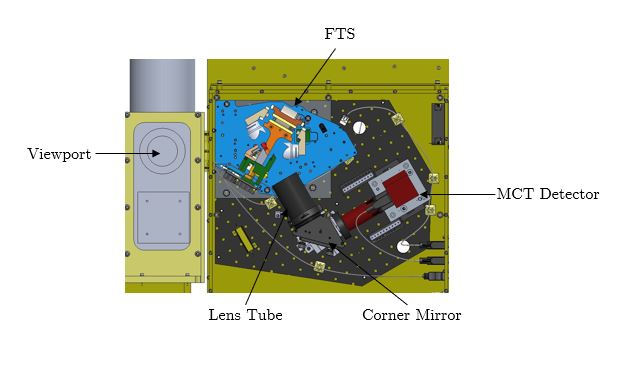
\includegraphics[width=\linewidth]{chap3_images/optical_system_diagram.JPG}
  \caption{LIFE optical system model}
  \label{fig:optical_system_diagram}
\end{figure}

The optical system consists of the FTS, the MCT detector, and the imaging lens system between the FTS and detector. The first consideration is that the detector must be operated at 70K or lower as typical of MCT detectors. This requirement is already met by the pre-installed Stirling Cooler that sits above the detector, so this requirement itself did not play heavily into the thermal design. However, something that still needs to be considered here is the removal of heat from this system. It must be ensured that the Stirling Cooler is able to remove heat from the detector and transfer that heat, either through conduction to the optics plate below or through sufficient radiation. Also as a result, this heat will warm other components nearby, and this must be considered as well.

The lens array and FTS are the components that need to be most carefully thermally controlled. For the thermal range of the system, temperature requirements are not as rigidly defined for operation as for electronics, but must be defined for environmental and mechanical reasons. Condensation in the lenses must be prevent during the ascent of the flight, where the instrument travels through a cold and humid troposphere. To provide a reasonably large margin so that the optics do not drop close to 0°C, a lower temperature requirement was set at 10°C. For the warm case, thermal expansion of the lenses are an issue, which may change optical properties and cause alignment issues. To avoid this the warm temperature requirement was set at 25°C. In addition to this temperature range, the temperature drift must be considered as well, as required to avoid issues with self-emission and removing the self-emission signal in the data analysis. As the time frame for multiple images of an instrument view (i.e. a blackbody, or the limb) is on the order of minutes, the drift must be as small as possible over this range; a requirement is set as less than 0.1°C/min temperature drift over the lens and FTS thermal systems. 

The mechanical requirements are to avoid any movement of any aspect of the optical system, at any point. The lens system is very carefully aligned, and it can be difficult to notice an issue with alignment as well as re-align the system, due to it being designed for non-visible light. The system must be as firmly built as possible to avoid any issues. Further, there was originally the requirement of removing vibrations from the system; small vibrations from the Stirling cooler were initially planned to be dampened or removed through some mechanical design. However, through discussions with ABB, it was eventually decided that these vibrations would not have enough of a detrimental effect on the data to require a much more complex vibration dampening optics system design, and was removed from consideration.

\begin{table}[h]
\begin{center}
\begin{tabular}{ |c|c| }
 \hline
 \rowcolor{lightgray}
 System & Requirement\\
  \hline
  \hline
  MCT Detector & Temperature at 70K\\
 \hline
  MCT Detector & Dissipate heat to avoid overheating\\
 \hline
 FTS/Lenses & Temperature between 10°C - 25°C\\
 \hline
 FTS/Lenses & Temperature drift $<$ 0.1°/min\\
 \hline
 Mechanical & Minimize vibration\\
 \hline
\end{tabular}
\end{center}
\caption{Optical system requirements}
 \label{optics_req_table}
\end{table}

\subsection{Electronics}\label{electronics_reqs}
The electrical components of LIFE have a wide variety of temperature ranges, which plays a large part in the design of the electronics box. There are a few particular components that have a narrow temperature range requirement, and it must be placed accordingly and verified with simulations. It is typical to place electronics in a seperate box from the optical system, for both cleanliness and thermal reasons. The electronics in LIFE do not need to be as carefully thermally controlled and kept as steady as the optics, but it must be ensured that they will not swing outside the required temperature range, especially during the ascent phase of flight through the tropopause. In particular, the most  thermally sensitive components are the control board for the FTS system (BMXS Board), and the ethernet interface boards (Pleora Boards) attached to the detector data acquisition boards. The thermal requirements for all major electronics in LIFE are detailed in Table \ref{therm_req_table}. 

\begin{table}[h]
\begin{center}
\begin{tabular}{ |c|c|c| }
 \hline
 \rowcolor{lightgray}
 Component & Minimum Temperature (°C) & Maximum Temperature (°C)\\
  \hline
  \hline
 BMXS Board  & 5 & 35 \\
 \hline
 CPU Stack (x2)  & -40 & 85 \\
 \hline
 DAQ Board (x2)  & -40 & 60 \\
 \hline
 DC-DC Converter & -40 & 85 \\
 \hline
 Ethernet Switch & -40 & 70 \\
 \hline
 Motor Driver & 0 & 60 \\
 \hline
 Pleora Board (x2)  & 0 & 40 \\
 \hline
 Temperature Controllers (x5) & -40 & 85 \\
 \hline
 VIPAC Power Supply & -40 & 95 \\
 \hline
\end{tabular}
\end{center}
\caption{Temperature limits of the major electrical system components.}
 \label{therm_req_table}
\end{table}

Connected to these requirements is for the instrument to be able to dissipate enough heat in the warm scenario, without freezing in the cold scenario. The power of each component is described later in Section \ref{prelim_design}, but overall the total dissipation of the instrument is upwards of 500W, largely due to the two DAQ boards of 40W each. The instrument must be designed to move this heat away from these boards quickly, and played a large role in the design.

\subsection{Mechanical}
The goal of the LIFE prototype was to fly on a high-altitude balloon gondola, and to be able to meet this goal the instrument had to meet mechanical requirements as outlined by CNES and the CSA. These requirements included volume, weight, bolt pattern, force and impact requirements. In addition to the gondola constraints, the instrument needed to be tested inside the ISAS Thermal Vacuum chamber, which provided further volume constraints. A summary of all requirements can be found in Table X.

\begin{figure}[h]
\centering
  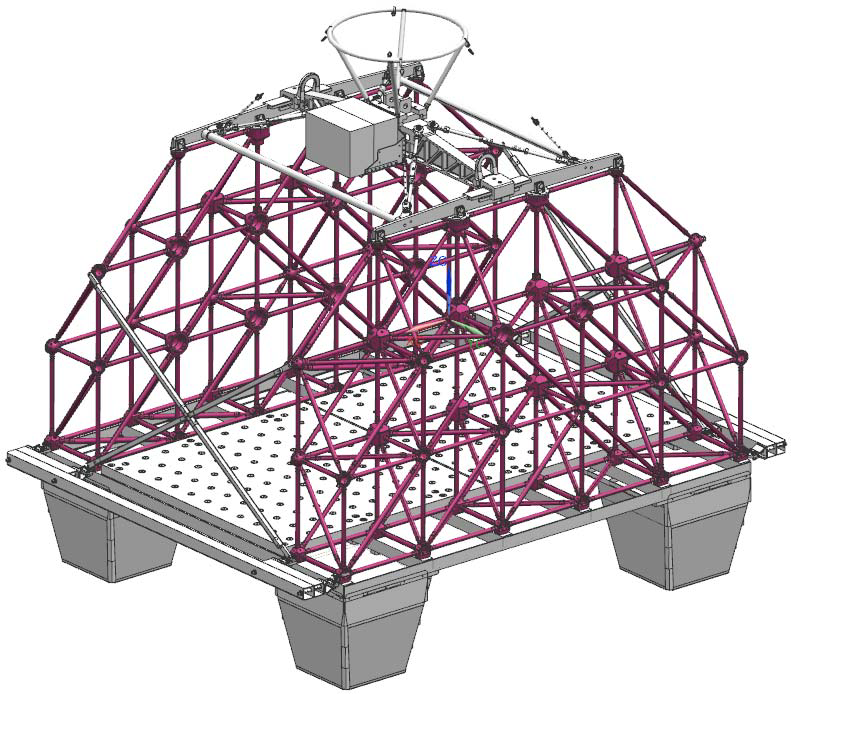
\includegraphics[width=0.7\linewidth]{chap3_images/Carmencita_empty.png}
  \caption{The CNES Carmencita gondola which carried LIFE for the test flight.}
  \label{fig:Carmencita_empty}
\end{figure}

CNES has multiple high-altitude gondola models of different sizes, and LIFE was designed to work with \textit{Carmencita}, the smallest model. A CAD model of Carmencita is shown in Figure \ref{fig:Carmencita_empty}. The design requirements that this gondola imposed upon the LIFE design were the volume, mass and bolt pattern constraints. As it is the smallest CNES gondola, and the flight was being shared with a few other smaller experiments, the CSA gave LIFE a weight requirement of no more than 100kg. In terms of size, the gondola is a modular design, forming 'boxes' with corner nodes that can be connected to other boxes. The size of one of these boxes is 342mm x 342mm, meaning that the total height of the gondola is 1.026m in the centre, sloping down to 342mm on the edge. No part of the instrument could protrude past this limit as a thermal blanket would be placed over top as a cover. LIFE was planned to be placed towards the centre of the gondola to maximize height allowance, but the sloping cover still needed to be taken into account depending on the width of the instrument. The honeycomb base plate panels that the instrument would attach to led to requirements for length and bolt pattern. The instrument base plate must match a 100mm x 100mm M6 pattern, and avoid protrusions used to attach the base plate to the structure. This gave a base plate length requirement of 950mm. The wall-to-wall length was slightly longer, at 1114mm~\citep{STRATOS_CARMENCITA_doc}. The TVAC chamber gives further volume requirements, with an internal size of 106 x 813 x 794mm. A more detailed overview of the TVAC chamber is provided in Section \ref{TVAC_tests}. Both these dimensions and the Carmencita dimensions provided an overall size requirement of 950 x 813 x 794mm. 

LIFE had to meet numerous mechanical requirements as specified by the CSA. They provided an extensive Excel document which would calculate forces at each interface of the gondola to ensure it would survive a worst case force scenario. This was calculated at multiple angles from 0° to 315°, and calculated the maximum shear and tension in force. A more detailed examination of these interfaces and forces calculated can be found in Section \ref{prelim_design}, as the survival requirements depended on the detailed design, including mass and bolt pattern. However, one of the defining values for survival was the maximum force due to acceleration or shock. For the weight and size of the Carmencita gondola, this was given as 15g shock at ground impact. Other forces included rapid deceleration after parachute opening, at 8g. As LIFE was relatively heavy, it had to be ensured during design and through simulations that the connection between the instrument and the gondola, as well as connections between various parts of the instrument would be able to survive as maximum shock of this magnitude.

\section{Thermal Environment}\label{thermal_env_ch3_sec}
In addition to the stringent requirements given for the electrical and optical systems, these requirements need to be met in numerous environments, subject to a variety of conditions. The instrument must be designed by simulating temperatures through different scenarios to ensure survival. This section discusses the main three environments the instrument will see, and the plan for simulations: the Lab, the ascent phase of the flight, and the main float part of the flight. These environments formed the basis of the simulation temperatures and environments. 

\subsubsection{Lab Environment}
The instrument is most often operating in the lab environment. An air conditioning unit was installed in the lab to ensure that temperatures of both the instrument and the room would not increase substantially. The average temperature of the room was measured before the thermal system of the instrument was designed, so that the lab case for thermal simulations, known as the \textit{warm} case, could be determined as having an atmospheric temperature of 20°C.

A difficult component of this environment is convection, which is difficult to model. As described in Section \ref{heat_transfer}, it is even difficult to just to estimate a reasonable starting point for values such as the convection coefficient, which has a large impact on the resulting temperatures. Since this would have caused to much uncertainty in the model, convection is ignored for the lab environment simulations. Although this does not make the simulations accurate, it provides a worst case scenario, as convection will only cool the instrument when the instrument is at higher temperatures than the room which is being cooled via air conditioning. Thus the baseline for the simulations was to set a temperature of 20°C and meet temperature requirements without the use of convection to cool. 

As a precaution for cooling, fans were also planned to be installed in the instrument. Ideally, the flow from these fans would cause forced conduction upon the electronics and cool everything quickly, and this could theoretically be modelled via the SolidWorks Flow Analysis package, which would allow the simulations to be more accurate for the lab environment. However the package was deemed too difficult to use for this purpose, and unless there were serious temperature issues with the radiation and conduction based lab simulations, it would not be used.

\subsubsection{Ascent}
Ascent is the most rapidly changing environment, and also provides a wide array of unknowns, making it difficult to simulate properly. Ascent covers the phase from when the instrument is launched to when it reaches float altitude, covering over 30km. Both temperature and pressure change rapidly in this region, and for the LIFE flight from Timmins a pressure variation from 1000hPa to 3hPa, and a temperature range from 10°C to -70°C as a worst case scenario. This minimum temperature can occur for as long as 60 minutes~\citep{STRATOS_CARMENCITA_doc}. These changes lead to difficulty in the simulation of convection, which depends on a number of variables, including temperature and pressure.

Due to the error in most simulation variables, this portion of flight was chosen not to be modelled before flight. From previous instruments, it was found that although the temperature drop through the ascent has a noticeable effect, it is not in this region long enough to freeze and damage electronics. Further, there are no papers or materials on with data on the change in convection in this pressure or temperature range; studies are typically done in warm environments at higher pressures, for the purpose of studying mechanical systems. It was decided that the instrument would be designed to withstand the worst case scold scenario at float altitude, and post-flight a simulation would be created based on the measured temperature through ascent, to inform future instruments and missions.

\subsubsection{Float}
At float altitude, the environment is fairly well defined and stable. Thus the instrument can be designed to survive and operate here with reasonable certainty in the simulation. Although the measurements of the LIFE instrument do not depend on the time of day or night, contrary to many atmospheric sensing instruments, it is chosen to fly at night to further define the thermal environment. It removes the possibility of seeing the sun, which presents issues such as solar heating and radiation, both of which are not well defined and are based on the viewing geometry of the instrument with respect to the sun, as well as what parts are shaded. In the night environment, the only external thermal impact on the instrument is due to conduction between the instrument baseplate and the gondola. As measured during the CATS flight and discussed in Section \ref{balloon_env}, the coldest the gondola will get is -40°C. This was used as the worst case cold scenario for the initial simulations. For the majority of the flight, the baseplate will sit between -20°C and -30°C, so the most common scenario, or the middle simulation case, was a baseplate at -30°C. In total, there are three initial simulation cases: 20°C (lab, warm case), -30°C (float, base case), -40°C (float, coldest case, following ascent). 

During flight, due to the unavailability of a landing site, the landing was delayed until the afternoon, well after the sun had risen. So even though the sun case was not considered in the design, it played a role in the resulting thermal data and should be described here. If a flight is planned to go past sunrise, sun shields are installed on the gondola to provide shade for the instruments to reduce solar heating. Solar heating at this altitude, due to the lack of atmosphere, can have a very strong impact on the temperature of an instrument if the absorptivity of a material is high. An example given from the CSA is a black anodized aluminum material, with an absorptivity $\alpha$ of 0.67, will reach a surface temperature of 117°C in direct sunlight of 1400 $W/m^2$ solar flux at float ambient temperature~\citep{STRATOS_CARMENCITA_doc}. Radiation will also be effected, as the object seen by the surface is at a very high temperature, as opposed to the cold atmosphere or deep space. The effects on LIFE of the part of the flight after sunrise is described and analyzed in Chapter \ref{postflight}.

Finally, the float component of the flight is good to simulate thermally as the simulations can be verified in the lab through the use of a Thermal Vacuum chamber (TVAC). With a vacuum environment and a cold plate that can reach -40°C through the use of liquid nitrogen, it can provide a very good simulation of the actual flight float environment. Comparing results of the simulation to the actual results of a TVAC can help determine the answers to a number of questions, such as basic survivability, but also unknowns such as heat transfer coefficients across gaps. A more detailed discussion on the LIFE TVAC tests can be found in Section \ref{TVAC_tests}.

\section{Thermal-Mechanical Design \& Simulation Software}\label{thermal_sim_sw_sec}
With previous instruments, the thermal requirements were not overly stringent, and the thermal design could be estimated with simple calculations and knowledge of previous missions. With the LIFE requirements it was determined that this would not provide enough accuracy for flight, and a full thermal analysis of the instrument was needed. A thermal model was to be created, based on the instrument mechanical model. It would analyze the thermal performance in different flight and lab environments, and determine the necessary methods required to keep the instruments above freezing as well as to dissipate enough heat. Both mechanical and thermal designs were iterated many times before coming to a final design solution. The software used to perform the analysis and design, is described here. This section also explains the basis behind many design analyses, Finite Element Analysis, and relates this to how this is used in LIFE thermal simulations.

\subsection{Computer Assisted Design Software}
There are a wide variety of Computer Assisted Design (CAD) software available, and they are all used widely in industry. A large subset of these can also perform thermal analyses within the program. Research was done into different software to determine which would best suit the needs of the LIFE simulations. Two final options were found: Siemens NX and SolidWorks, both the most popular options in industry.

Siemens NX, developed by Siemens AG, is a CAD software heavily used throughout industry for advanced modelling of large designs, and particularly thermal simulations. It was recommended for the LIFE project by Honeywell Aerospace, which it used to develop the thermal model of the CATS and ALI instruments that the ISAS group has co-developed. Their thermal modelling software is widely considered the most advanced in the industry, particularly in aerospace design. However, downsides to NX are a very steep learning curve and price, due to its depth. Regardless, the thermal simulation software would likely be the best to suit the needs of LIFE.

SolidWorks, developed by Dassault Systems, is likely the most popular CAD software available. It is designed more for modelling of smaller designs and parts rather than large assemblies, and has overall less functionality. While this is a downside, it also has an easier learning curve, and academic licenses are easily available, which cuts down on cost. Due to its popularity, there is a large amount of community support through forums and online tutorials on both its basic functionality and simulation abilities. Further, the early initial CAD model of LIFE had already designed in SolidWorks; using the thermal analysis functionality of the program would be much simpler, not having to rely on exporting to another software. The thermal simulation suite, which comes built-in with an academic license, does not have the depth in NX, which would lead to less accurate simulations. SolidWorks does have an electronics thermal modelling package as an add-on, which would be beneficial to the design. However the complexity of the package was larger than was necessary, and was not considered in the final decision. Overall however, due in large part to the much cheaper cost and prior experience in the software, SolidWorks was eventually chosen to be used for the simulations and to develop the CAD model further. 

The mechanical model for LIFE, as is described in depth in Section \ref{prelim_design}, is designed entirely using SolidWorks. The thermal design is discussed in tandem with the evolution of the mechanical design, as they are heavily connected. Simulations were done with the aforementioned built in thermal software, as well as some structural simulations as well. The basis behind all SolidWorks simulations is an analysis technique known as Finite Element Analysis.

\subsection{Finite Element Analysis} \label{FEA}
Finite Element Analysis (FEA), also sometimes referred to as the Finite Element Method (FEM), is one of the most important numerical analysis tools available for engineering design. It allows any arbitrary surface or shape in any number of dimensions to be analysed and simulated numerically. This method works with materials that are anisotropic, and the simulated sources (i.e. force or heat) do not need to be overly specific. Almost all CAD software simulations utilize FEA at its basis. FEA, overall, is a process of converting any shape along with its sources and restraints that can be represented by differential equations to a system of matrices that can be solved to give an approximate solution~\citep{FEA_SW}.

The basis of FEA is to replace any complex shape or model with simple shapes, that when summed together create the original shape. These simple shapes, which are dependent on the simulation but most often some type of triangle, are known as finite elements. These can be compared to the original model in the same way that finite elements of a sum can be compared to infinitesimal differential elements of integral equations. The elements can be altered in numerous ways, including shape and size, to work best for each simulation~\citep{FEA_SW}. The array of elements when it is applied to a part is known as a mesh. An example of a shape being converted into both a coarse mesh and fine mesh with slightly different shapes is shown in Figure \ref{FEA_mesh_example}.

\begin{figure}
    \centering
    \begin{subfigure}[h]{0.6\textwidth}
        \centering
        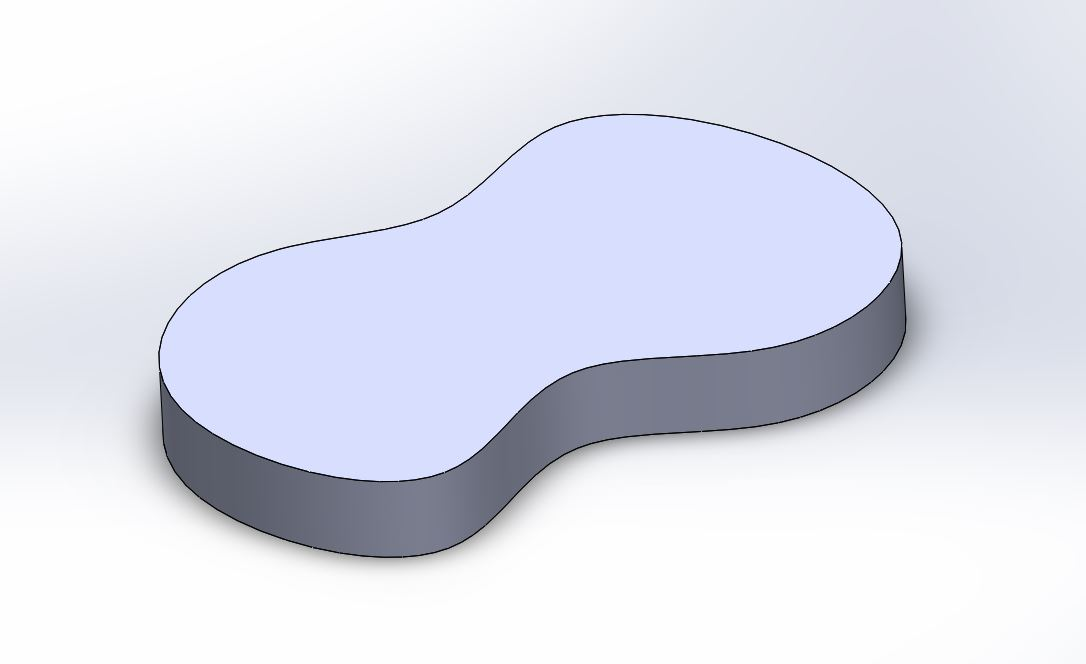
\includegraphics[width=\textwidth]{chap3_images/mesh_test_part_no_mesh.JPG}
        \caption{Example SolidWorks part, before elements applied.}
        \label{fig:FEA_mesh_before}
    \end{subfigure}
    \begin{subfigure}[h]{0.6\textwidth}
        \centering
        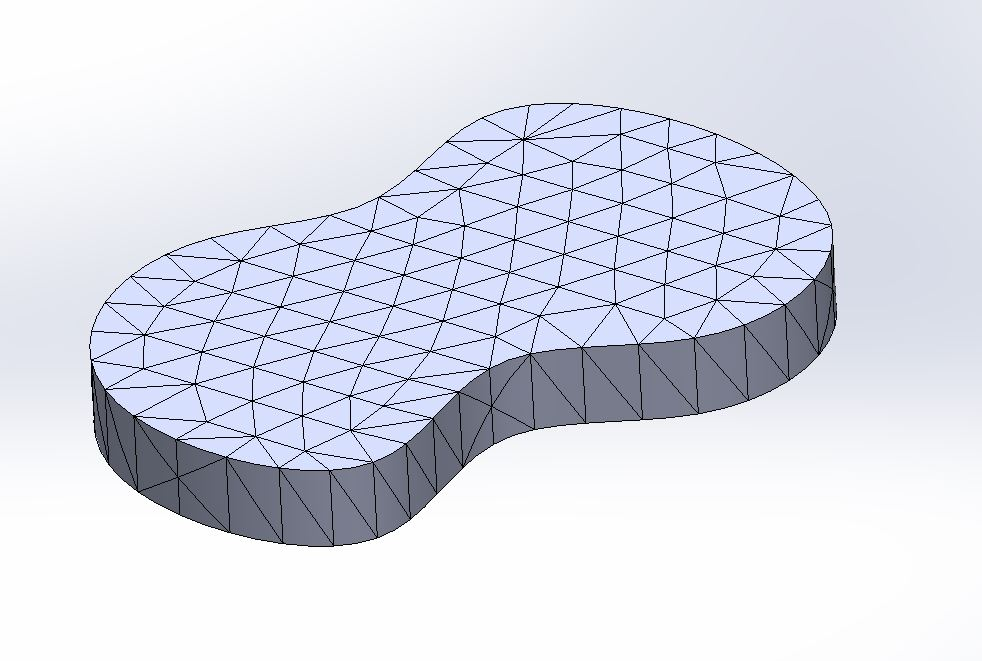
\includegraphics[width=\textwidth]{chap3_images/mesh_test_part_coarse_mesh.JPG}
        \caption{Example SolidWorks part, with coarse, regular elements.}
        \label{fig:FEA_mesh_coarse}
    \end{subfigure}
    \begin{subfigure}[h]{0.6\textwidth}
        \centering
        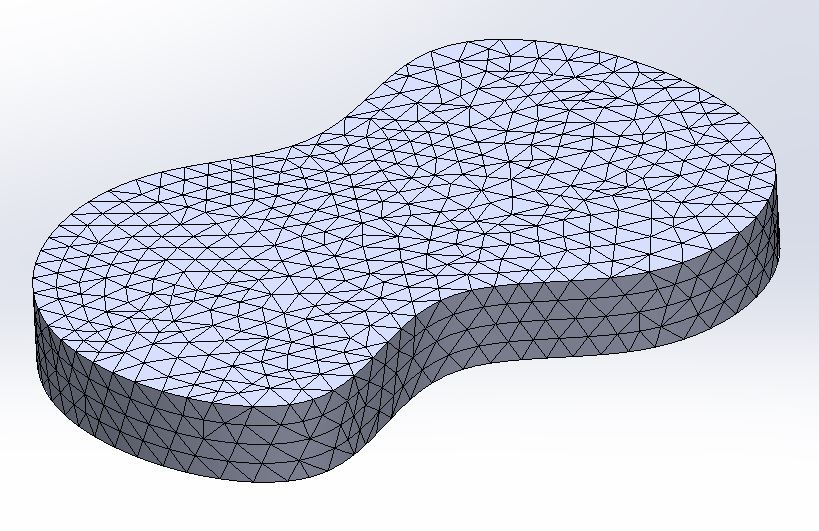
\includegraphics[width=\textwidth]{chap3_images/mesh_test_part_fine_mesh.JPG}
        \caption{Example SolidWorks part, with fine, curved elements.}
        \label{fig:FEA_mesh_fine}
    \end{subfigure}
    \caption{A shape being converted to finite elements, or a mesh.}
    \label{FEA_mesh_example}
\end{figure}

The volume of this part could now be easily calculated. The choice of element shape must be considered when creating the mesh; Computationally, the linear triangle, as shown in Figure \ref{fig:FEA_mesh_coarse}, is easiest to solve using a simple area equation for a linear triangle. All that is needed is the vertex components for all triangles to be able to calculate the area or volume. A quadratic triangle with curved sides, as shown in Figure \ref{fig:FEA_mesh_fine}, is better at approximating curved shapes, however more advanced numerical integration is needed to solve for the area or volume of a quadratic triangle~\citep{FEA_SW}. It is a trade-off that must be considered between error and simulation solve time, but often there is no choice, especially working with a lot of curved components, that the latter and more computationally expensive option must be used. By default, SolidWorks uses quadratic triangles, but may go to higher polynomials if necessary. A volume element is always uses tetrahedral elements for volume components. 

The evaluation of an FEA problem relies heavily on the mesh, and particularly its vertices. The mesh generates two arrays: The first is a list of all vertices, with their spacial coordinates, and is known as the nodal set. The second is known as the connectivity list and describes each vertex along with the vertices that it is connected to. This list is critical to solving analyses and simulations, as these inform the matrices and equations used for the solution~\citep{FEA_SW}. For each vertex in the mesh, there is one simultaneous equation that describes every equation or variable that may impact the final values at that node. 

For whatever type of simulation is being done, the general equilibrium matrix will always be the same. It is simplest to show this with the well known spring system, following the example in the textbook \textit{Finite Element Analysis Concepts via SolidWorks}. For the problem of a single spring that is generalized so that either side can be restrained or loaded with force, the equilibrium equations can be shown as the matrix form in Equation \ref{spring_FEA_matrix}.

\begin{equation} \label{spring_FEA_matrix}
\begingroup
    k
    \begin{bmatrix}
        1 & -1 \\
        -1 & 1
    \end{bmatrix}
    \begin{Bmatrix}
        u_1 \\
        u_2 \\
    \end{Bmatrix}
    =
    \begin{Bmatrix}
        f_1 \\
        f_2 \\
    \end{Bmatrix}
\endgroup
\end{equation}

Here $k$ is the stiffness, $u$ is the displacement, $f$ is the force, and the subscripts corresponds to each side of the spring. This can be used to represent a node of the matrix. However, this form the equation cannot be solved; there is only information about this one node. Information must be given as an initial condition, i.e. displacement, and boundary conditions, i.e. force. If the initial condition is given as $u_given$ and the force on one end of the spring is given as $F$, the Equation \ref{spring_FEA_matrix} can be written as Equation \ref{spring_FEA_matrix_solvable}.

\begin{equation} \label{spring_FEA_matrix_solvable}
\begingroup
    k
    \begin{bmatrix}
        1 & -1 \\
        -1 & 1
    \end{bmatrix}
    \begin{Bmatrix}
        u_{given} \\
        u_2 \\
    \end{Bmatrix}
    =
    \begin{Bmatrix}
        F \\
        f_2 \\
    \end{Bmatrix}
\endgroup
\end{equation}

This leaves the displacement of the other end of the spring and the reactionary force to be solved for. The two given values would be input into SolidWorks, say as the force on a plate and its initial displacement, and it would calculate how far the next node would move based on its force and displacement from the initial node. This is calculated for all nodes in the mesh. This equation becomes much more complex as more nodes are added and as the shape of the elements becomes more complex, leading to more inputs on each node from other nodes. The general equation for the mechanical displacement problem is given in Equation \ref{gen_FEA_matrix}.

\begin{equation} \label{gen_FEA_matrix}
\begingroup \boldmath
    \begin{bmatrix}
        K_{uu} & K_{ug} \\
        K_{gu} & K_{gg}
    \end{bmatrix}
    \begin{Bmatrix}
        \Delta_u \\
        \Delta_g \\
    \end{Bmatrix}
    =
    \begin{Bmatrix}
        F_g \\
        F_u \\
    \end{Bmatrix}
\endgroup
\end{equation}

Here, $bm{\Delta_u}$ are the unknown nodal displacements, $\bm{\Delta_g}$ are the given boundary values of other displacements, such as a restraint on the edge boundary of a part. For a known part, all values of the $\bm{K}$ matrices are known. The applied loads to the nodes is represented by $\bm{F_g}$, with $\bm{F_u}$ as the unknown reaction forces from other nodes and their boundary conditions. As there are only two unknowns remaining, this general matrix can be solved. 

Structural and thermal analysis have a number of analogous terms, making it simple to use Equation \ref{gen_FEA_matrix} in thermal simulations be changing a few variables. A table showing the conversion from structural analysis to thermal analysis is shown in Table \ref{mech_to_thermal_properties}~\citep{FEA_SW}.

\begin{table}[h]
\begin{center}
\begin{tabular}{ |c|c|c| }
 \hline
 \rowcolor{lightgray}
 Equation Component & Thermal Variable  & Mechanical Variable\\
  \hline
  Unknown & Temperature, T [K] & Displacement, u [m]\\
  \hline
 Gradient & Temperature gradient, $\Delta T$ [K/m] & Strain, $\epsilon$ [m/m]\\
 \hline
 Flux & Heat flux, q [W/m\textsuperscript{2}] & Stress, $\sigma$ [N/m\textsuperscript{2}]\\
 \hline
 Source & Heat source, Q [W] & Force, g [N]\\
 \hline
 Indirect restraint & Convection & Elastic Support \\
 \hline
 Restraint & Set temperature, T [K] & Set displacement, u [m]\\
 \hline
 Reaction & Heat flow, H or Q [W] & Force, F [N]\\
 \hline
 Material Property & Thermal conductivity, k [W/mK] & Stiffness, k [N/m\textsuperscript{2}]\\
 \hline
 Law & Fourier's Law & Hooke's Law\\
 \hline
\end{tabular}
\end{center}
\caption{Equivalents between thermal and mechanical simulations}
 \label{mech_to_thermal_properties}
\end{table}

Thermal simulations with FEA all have a single equation governing each node, as in mechanical simulations. All above components of the equation are considered within this equation. This includes heat flux due to heat power, radiation, and conduction, the convection restraint, restraints on specified temperatures (for example, the base plate must be -40°C as a worst-case scenario), the reactions are the resultant heat flow that is necessary to maintain the specified temperatures, and the final unknown is the temperature. All other conditions add source terms, such as the dissipated heat power of electrical components~\citep{FEA_SW}.

For thermal equilibrium, the resulting matrix equations have a general form as shown in Equation \ref{gen_T_matrix}.

\begin{equation} \label{gen_T_matrix}
\begingroup \boldmath
    \begin{bmatrix}
        K_{uu} & K_{ug} \\
        K_{gu} & K_{gg}
    \end{bmatrix}
    \begin{bmatrix}
        T_u \\
        T_g \\
    \end{bmatrix}
    =
    \begin{bmatrix}
        F_g \\
        F_u \\
    \end{bmatrix}
\endgroup
\end{equation}

where $\bm{T_f}$ represents the restrained vertex temperatures and $\bm{F_g}$ represents the thermal heat power (heat flow) of the vertex. The $\bm{K}$ values represent the thermal conductivity matrix for each node, where if the material is assumed isotropic will be a unit matrix. $\bm{F_u}$ is unknown and represents the total heat flow in or out of a node that is necessary to maintain the given temperatures $\bm{T_g}$. $\bm{F_g}$ is calculated with heat flux, which is where conduction and radiation equations are used in the solution. For thermal conductive heat flux, Fourier's Law is used, from Equation \ref{FC_law}. Heat flux incident on the body and radiation from the body is from Equation \ref{SB_surroundings}. $\bm{F_u}$ is thus calculated from adding the conductive flux from Equation \ref{FC_law} the radiation flux from Equation \ref{SB_surroundings}, and the flux resulting from $\bm{F_g}$. This allows to complete the goal of the equations which is to solve for $\bm{T_u}$~\citep{FEA_SW}~\citep{FEA_Procedures}. An example solution equation for the temperature at a node would look like Equation \ref{TA_solution_eq}.

\begin{equation}\label{TA_solution_eq}
    \bm{T_u = K_{uu}^{-1}(F_g-K_{ug}T_g)}
\end{equation}

In a simple example part in a vacuum environment, $\bm{T_g}$ would be an array of constants as chosen for the simulation, k would be a constant if the material was isotropic, and $\bm{F_g}$ would the conductive heat flow plus the radiative heat flow. 

The size of the set of equations that is in general given by Equation \ref{gen_FEA_matrix} is the number of nodes. Thus, for an example of 100,000 nodes, there are 100,000 equations, and 100,000 temperatures calculated. Putting all these nodes together on the CAD model gives a solved thermal model necessary for thermal analysis.  The model can be evaluated for both lab and flight conditions by including or neglecting convection respectively, and by specifying relevant boundary conditions. 

\section{Preliminary Thermal-Mechanical Design}\label{prelim_design}
The preliminary design for LIFE was completed using SolidWorks, through a series of iterations of different components of the instrument. It is one of the core parts of this thesis. In all, the instrument can be split into four major parts: The blackbody system, the box containing the optical system, the main electronics box which contains electrical parts for the FTS and detector as well as the computers, and finally a smaller electronics box that contains the electronics used to control the blackbodies. To give an overview for how these parts are connected before going into detail of the design process for each, a block diagram of LIFE is provided in Figure \ref{fig:LIFE_block_diagram}.

\begin{figure}
    \centering
    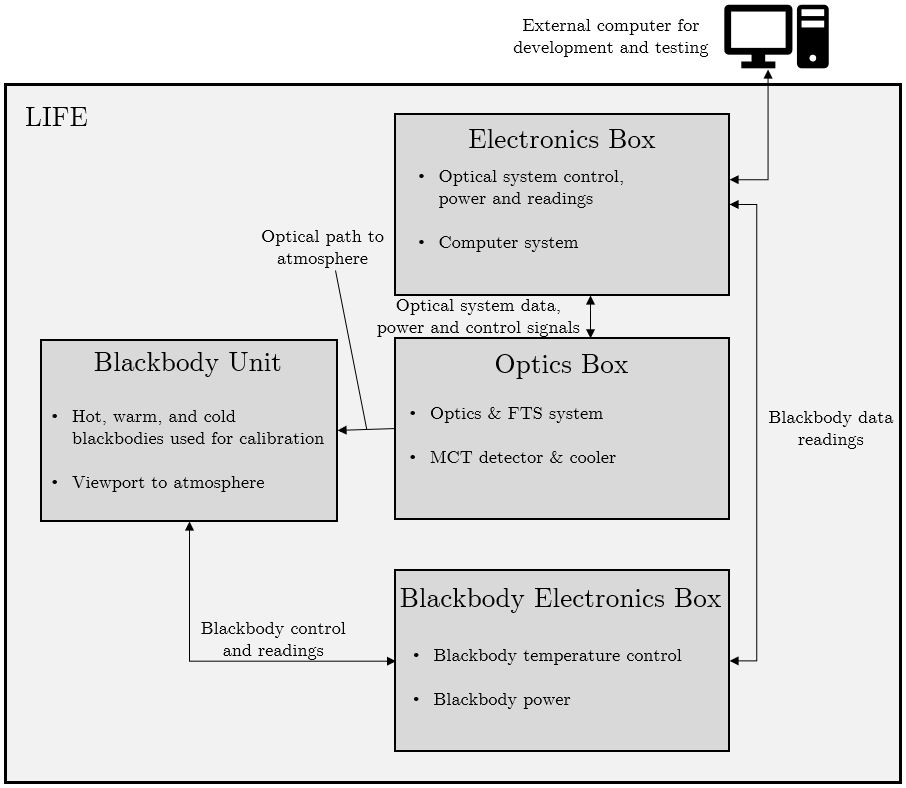
\includegraphics[width=\linewidth]{chap3_images/LIFE_block_diagram.JPG}
    \caption{Block diagram of the LIFE instrument.}
    \label{fig:LIFE_block_diagram}
\end{figure}

Although there are fluctuations through the design process, it is helpful to give an overview of the purpose of each component. The blackbody assembly houses the three blackbodies that the instrument images during calibration and testing, which was procured from ABB. The instrument also views the atmosphere through this unit, through a side viewport. This system is described in greater detail in Section \ref{blackbody_assem_sec}. The optics box houses all the core components of the imaging system of the instrument: The lens array, the FTS, and the detector. These are all mounted to a optical breadboard plate, which is mounted to the side of the inside of the box for FOV purposes. The optical path goes out a window into the blackbody unit, where it is reflected into the atmosphere. The electronics box houses the parts necessary for operation of all components of the instrument, except for the blackbodies. This includes the data acquisition boards for the detector, the control board for the FTS, the computer system, multiple power supplies, and its own heaters and temperature controllers. As such, there are critical connections between the optics and electronics box that carry the sensitive data signals from the detector as well as control signals to and from the FTS. This box also interfaces with an external computer, which can be used if necessary to control and read data from the instrument during the development and testing phase, as well as troubleshooting. Finally, the blackbody electronics box houses the electronics necessary for operation of the blackbodies, such as the temperature controllers and power supply. In early iterations, the electronics in this box were part of the main electronics box, until the size grew too large for the volume requirements of the CNES gondola. It sends this data to the main computer in the electronics box.

The LIFE instrument went through a large number of design iterations before reaching the final design that was constructed and launched. Each subsection below, with the exception of the Blackbody Assembly (as it did not play a role in the design iterations), discusses a version of the design. This includes a detailed description of the optics and electronics boxes, which each went through a number of their own versions, and the thermal analysis donefor each. The thermal analysis often formed the basis for a new version of the design. The final section goes into further detail about the final version and the detailed thermal analysis that was done to prepare it for TVAC tests and the flight.
%Trying to split the sections into a bit more organic order. Subsubsections may not be necessary for each, it will depend on length, could also add a 'full assembly' section at the end, depending necessary length. Could also split by mech and thermal/
\subsection{LIFE Preliminary Design: Blackbody Assembly}\label{blackbody_assem_sec}
The blackbody assembly, unlike the rest of the design, was not designed in-house. It was procured separately from ABB for use in the LIFE instrument, to save the cost of designing and building, or purchasing, a new blackbody system. However, it still required work to characterize the blackbodies to ensure proper operation and to ensure that they would work properly with LIFE. They also play an important part in the overall LIFE design, so they will be described here before going further into the LIFE design.

The blackbody assembly has six blackbody surfaces that can be imaged, split into two halves. The original purpose of the instrument required two identical systems, so there are two viewports, three pairs of blackbodies, and two viewports towards the atmosphere. LIFE only requires one system, so the other was used only for lab verification testing. Focusing now on one part of the system, there are three surfaces that can be imaged. One is connected to a thermoelectric cooler, and is thus used as the cold blackbody. The minimum temperature of this cooler is unknown, but is rated to go well below zero degrees. However, in a lab environment, a surface temperature dropping below zero would lead to frost buildup on the surface, causing changes in the emissivity. With changes in the emissivity, the temperatures would no longer be measured properly, and in addition the frost buildup could cause dust and other materials to build up on the surface, rendering it less accurate. Thus the lowest temperature this blackbody was set at was 5°C, however it was set to 10°C for the majority of our testing. Another external blackbody, from the ACE instrument, was procured from ABB for the purposes of looking at a temperature well below freezing, in a TVAC environment. This is described in greater detail in Section \ref{non-linearity_sec}. 

The other two surfaces can theoretically be used interchangeably as the hot and warm blackbody surfaces, however it was discovered that the power of the heater inside the one surface is much larger than the other, so to ensure enough power to reliably keep the temperatures steady, the former was chosen as the hot blackbody surface. During tests, the blackbody surfaces were interchanged, and in a cold environment there is not enough power to keep the temperature steady of the hot blackbody with the lower power heater. Again, no maximum temperature was given for these surfaces, but were used in their original configuration as high as 225°C. In the LIFE configuration, most often the hot blackbody was set at 60°C and the warm blackbody was set at 30°C. An schematic of the blackbody system is shown in Figure \ref{fig:bb_schematic}, and an image of the  system is shown in Figure X.

\begin{figure}
    \centering
    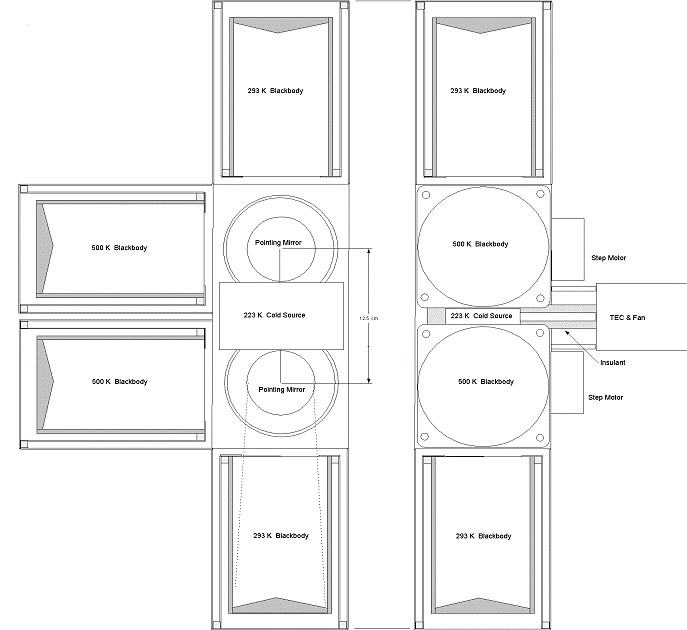
\includegraphics{chap3_images/Blackbody_schematic.png}
    \caption{Schematic of the LIFE Blackbody System.}
    \label{fig:bb_schematic}
\end{figure}
% ADD BLACKBODY SYSTEM FIGURE

The temperatures in the schematic show the temperatures from the original configuration, not the LIFE configuration. Also, for the final flight configuration of LIFE, it is noted that the bottom warm blackbody and the bottom hot blackbody are removed, as they are only used for lab verification and it is unnecessary weight. Plates were built and installed to cover the openings into the system left by removing these two blackbodies.

The blackbody system operates using a rotating mirror at the centre of each system. The optical path goes through the input window, and reflects off the mirror in whichever direction is necessary: Up for warm blackbody, right for hot blackbody, down for cold blackbody, and left towards the atmosphere. The optical properties of this mirror are unknown, which caused some uncertainty in the self-emission calculations. However as it has a gold coating and was used in a previous application where self-emission minimization was also important, it is assumed to be quite low. The operation of the mirror was done by rotating a stepper motor, which was one of the first parts of the system to be reconfigured for LIFE. Software needed to be developed to control the stepper motor, this was first done in the proprietary software interface for the particular stepper motor, which was used for all testing and development. Later, in-house software was developed using C++ to allow more direct control and avoid the use of the software interface. 

The accuracy of the stepper motor also needed to be verified for proper data analysis after flight. To allow retrievals of the data, a very precise knowledge of the viewing angle of the instrument was needed, to within 0.1°. As there was no encoder for the stepper motor, it was impossible to tell through data feedback where the motor exactly was; numerous measurements needed to be taken to see the variation in angle each time the mirror realigned itself to image a blackbody or the atmosphere. This also led to the discovery of a few systematic errors, such as the motor would overshoot its required stopping position by a certain number of steps. Through testing and development of the motor, this systematic error was corrected, and the error in angle was deemed to be within the 0.1° required.

The largest issue with the blackbody system that required characterization correction were the surface temperatures. Although the surface temperatures of the blackbodies were not important to the detector characterization, as long as it was well known and replicated in all images, the temperature drift over time of the surface was. The LIFE FTS system requires 2.3 seconds to take a full image; if the temperature of the imaged surface changes significantly during this time, there are significant errors in the spectral data and the results are meaningless. The blackbody temperatures must be kept as steady as possible during the image capture time, ideally less than 0.1°C. Temperatures of the blackbodies were controlled via Team Wavelength proportional–integral–derivative (PID) temperature controllers, which were able to withstand a vacuum environment with small modifications, and had been used by previous atmospheric research instruments developed by ISAS. It was discovered that when using these controllers with defined setpoints, the temperature would oscillate around the setpoint indefinitely. PID controllers reach their setpoints by oscillating around a setpoint making small corrections, with the oscillations becoming smaller and smaller until the steady setpoint was reached. In the LIFE design the setpoints would never be reached, and a different size of oscillation occurred for each blackbody: The hot blackbody oscillated by roughly 4°C every ten minutes, while the cold blackbody could oscillate by as much as 25°C in the same time frame. A temperature reading acquired by the warm blackbody temperature controller is shown in Figure X.

% ADD EXCEL PLOT OF OSCILLATING BLACKBODY TEMPERATURE

Often, in a PID system, the oscillation and setpoint overshoot can be minimized by selecting optimized P, I, and D values. In this temperature controller, the only value that allowed direct control through a dial was the proportional gain, P. However, tests with various values of proportional gain found it to have very little effect on the oscillation error. Eventually it was found through examining documentation and contacting the manufacturer that the integration constant can be changed by changing the capacitance in a part of the circuit, which involved changing a capacitor. The manufacturer could not provide any guess on what a better capacitance would be, only that it should be lower. Starting with a capacitance of 0.05{\textmu}F, different capacitors were tested with decreasing capacitance. With each decrease in capacitance, the oscillation decreased, but it was not until a 1nF capacitor was used that the error in temperature oscillation was within the required 0.1°C, for both the warm and hot blackbodies. However, even at this capacitance, the cold blackbody temperature continued to oscillate by as much as 2°C. This probablem was eventually solved by using a different temperature controller; this option was not easily available for the other two surfaces as they had to be used during flight and needed to be remotely controlled and to survive a vacuum environment. The cold blackbody was only to be used for verification in the lab, so the controller did not have the same requirements. An external controller was sourced, in which the PID values could be easily configured. Through further testing, the values were optimized such that the oscillation of the cold blackbody surface was 0.1°C. With the temperature drift requirements met for all three blackbodies, the blackbody system was fully ready to be used for LIFE.

\subsection{LIFE Preliminary Design: Version 1} % This needs to be written better, but I have no idea how
Prior to the beginning of my thesis, Ethan Runge had planned to develop the thermal-mechanical design himself as part of his MSc. Eventually, it was decided that due to the required amount of work for the design, it should be a separate thesis. However, prior to this decision and prior to my work, a first preliminary version was developed. A large part of Ethan's MSc. thesis was the development of the LIFE optical system, and a CAD model of this system had already been developed in SolidWorks partly through some of Ethan's work and partly from models sent by ABB. This was placed into two early versions for the optics and electronics boxes, both known as Version 1. Though these models would be eventually redesigned from the ground up as part of this thesis, besides the core optical system, it is helpful to examine this initial design as it would inform the basic concept of future designs. A model of LIFE Version 1 is shown in Figure \ref{fig:LIFE_V1}.

\begin{figure}[h] % Should be updated to the correct LIFE V1
    \centering
    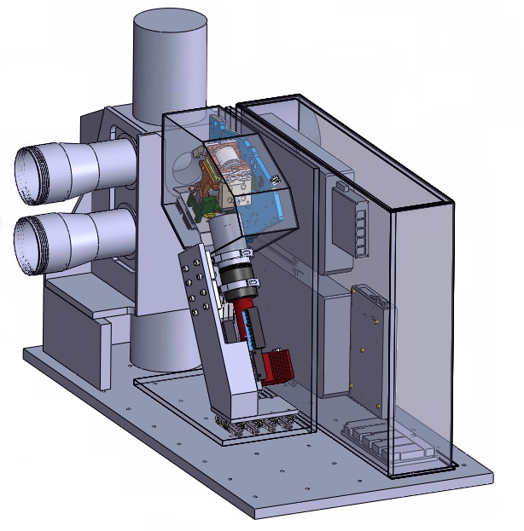
\includegraphics{chap3_images/LIFE_V1.png}
    \caption{LIFE Version 1, developed by Ethan Runge.}
    \label{fig:LIFE_V1}
\end{figure}

The layout of this design is the basis of the layout of all subsequent designs - a baseplate with the blackbody at the front, an box containing the core optical system that looks into the blackbody system, next to an electronics box that contains the optics electronics. However, this is the only aspect of the design that does not change through the subsequent iterations and updates. This footprint is heavily based on the requirement that the MCT Detector be tilted 90° relative to the horizontal, which is described in the next section.

\subsubsection{Optics Box Design: Version 1}
The driving requirement behind a optics box design where the optical system is mounted perpendicular to the baseplate against the box wall is due to the orientation of the MCT Detector. To vertically image the atmosphere, as is one of the goals of LIFE, the pixel array needed to be vertical. However, the detector that is supplied with the ABB system has a horizontal 1x16 pixel array. As a result, it needed to be mounted on its side, such that the horizontal array would be turned vertical, so the atmosphere could be vertically resolved. This was a break from all previous instruments that the ISAS atmospheric research group had designed, and required a vertical optics box. This also had further complications - it needed to be mounted to the wall, yet all parts needed to be free to move if necessary for alignment, and still be able to be sturdy to avoid any shaking causing miss alignments following the flight ascent. Version 1 of the optics box, designed to meet the requirement of tilting the detector and indeed the entire optical system, is shown in Figure X.

% ADD OPTICS BOX V1 IMAGE HERE (REALLY V0 - YOU KNOW WHAT I MEAN) - CAN ALSO TALK ABOUT DIFFERENT COMPONENTS OF THE OPTICS BOX HERE - SHOULD BE LABELLED.

The initial design used a construction material known as \textit{T-Frame}. It is an inexpensive, off the shelf component made from aluminum that is designed to easily fit together with other pieces of T-Frame and fasteners and connectors, all easily available and easy to build. Being able to order this material and build it in-house would save a large amount of the instrument budget. It also still allowed freedom in the design, as all components could be easily cut to length. Using a CAD model of this material taken from a suppliers website, a model for the box could be quickly designed. However, downsides to this material was that although easy to build, it was not entirely secure. As a result of manufacturing tolerances, each piece of the box could be loose connected to other pieces. Connecting things to this frame would also be a challenge, as there was no easy way to mount any parts, such as the FTS, to the wall, without having either an interface plate or to install it prior to putting the box together, which would lead to a large amount of time necessary for repairs.

Initially, as described in Section \ref{electronics_reqs}, vibration needed to be dampened as much as possible, due to the initial worry of vibrations from the Stirling cooler causing vibrations in the FTS, which may cause errors in the data. An idea to solve this was to use a spring system between the detector and the wall of the box, which would dampen the vibrations enough that they would not travel to the FTS system. The box was further stiffened through the use of rods connecting the two walls of the box. 

When I began my thesis, and took over the mechanical design, one of the first things that was determined was that the vibrations were not going to be as much of an issue as originally thought. As a result, the spring system and cross-braces were removed, as stiffness was not considered to be as much of an issue either. A Version 1.1 was developed, which was a simplified version of the original design with the optics attached to the walls and other unnecessary stiffening and dampening components removed. As thermal analysis was going to be one of the driving aspects of the design, the first thermal analysis of the model was done to this version of the optics box, by adding a heater to the T-Frame wall and measuring its effect. The results of that thermal model are in Figure X.

% ADD THERMAL MODEL OF OPTICS BOX V1.1

% TALK ABOUT THE RESULTS OF THIS ANALYSIS.

One of the main criticisms of this design is that it is open; the optics must be kept as clean as possible, and need to be well protected when not in a clean room. In addition, thermal control of the optics would be easier if the entire environment inside the box could be kept steady, rather than just a heater nearby in an open environment. Therefore, the main requirement of the next version of the optics box would be to design an enclosure for the optics, in a way that would enclose the optics and FTS while not directly attaching to anything and being easy to install around the optics. 

\subsubsection{Electronics Box Design: Version 1}
The design of the electronics box changes throughout the design process largely in part to two reasons: The thermal requirements, and adding more parts. As the mechanical design progressed, so did the electrical design, done by lab engineer Paul Loewen. This required room for more parts, and the box grew, and parts shifted around. However, for the first design, the only electronics that were of concern were the components necessary for the operation of the optical system: The FTS control board, known as the BMXS board, the two data acquisition boards, with the Pleora Ethernet interface boards attached, an Ethernet hub to allow the data acquisition boards, the BMXS board and the external computer to all communicate, and a power supply for the system. An image of Version 1 of the Electronics Box is shown in Figure X.

% ADD EBOX V1 FIGURE HERE
% MAY WANT TO TALK ABOUT T-FRAME HERE TOO, I CAN'T REMEMBER IF THIS VERSION HAD T-FRAME OR NOT (PROBABLY).
Although later in the process the design of the electronics box would be driven by the thermal analysis, the initial design was driven by the cables length connecting the detector and the data acquisition boards. Sixteen cables, one for each detector pixel, sent signals from the detector to these boards, to be amplified, digitized and sent to the computer. These cables were extremely delicate and could not be lengthened, due to the signals being unamplified coming from the detector, they would have to be fed directly from the optics box to the electronics box. Thus these boards were placed and oriented in the electronics box to minimize distance to the detector. The rest of the components were placed around arbitrarily in the rest of the box. Thermal analysis of this box would not be completed until the second version of this box when it had been converted to T-Frame and a few more components were added. With the use of thermal analysis, the components were placed differently according to their required temperature ranges.

\subsection{LIFE Preliminary Design: Version 2}
First updated version of LIFE, that I worked on: Optics box is at V1. Ebox is the same (double check), so don't need to add an electronics box section.

\subsubsection{Optics Box Design: Version 2}
Talk about first official update of optics box: Rearranged t-frame (made it shorter to cut out extra space, while still aligning with blackbodies) and added radiation plates.

\subsection{LIFE Preliminary Design: Version 3}
Second major update of LIFE, where the optics box is overhauled to follow cats design - Optics Box V2. Ebox is at V1 if it was not already at V1 over V0 (again double check) but probably does not need to be its own subsubsection.

\subsubsection{Optics Box Design: Version 3}
This version of the optics box was updated following CATS.

\subsection{LIFE Preliminary Design: Version 4}
Check if there were any updates to the optics box design, if there are it would only be a 2.1 upgrade. The main thing here is the ebox, which is updated to version 2.

\subsubsection{Electronics Box Design: Version 2}
This version of the electronics box was updated to not use T-Frame, similar to the CATS and optics box designs but without radiation plates.

\subsection{LIFE Preliminary Design: Version 5}
The current design. Only go through the initial design changes here though (i.e. the addition of the blackbody electronics box, no changes to the optics box), and go into full detail about it after all other designs have been discussed.

\subsubsection{Electronics Box Design: Version 3}
Go into detail about how some electronics needed to be added to this box, so some were transferred to a new box for space reasons. Could add blackbody electronics box as its own subsub section, but unlikely.

\subsection{LIFE Preliminary Design: Version 6}
This was the weird design where we started transfering different things between eboxes, making two similarly sized eboxes.

\subsubsection{Opto-Electronics Box: Version 1}
This added all the optics electronics to one box by themselves.

\subsubsection{Electronics Box Design: Version 4}
Smaller size for the main electronics box, now that the optics electronics (i.e. BMXS, Pleoras) are in their own box by themselves.

\subsection{LIFE Preliminary Design: Version 7}
Final new version, this was designed to be tilted for the appropriate field of view. Had a concept of an Optics Box V3, which would have either a tilted base or a tilted thor labs plate, but (luckily) this was scrapped not too far into development.

\subsection{Final LIFE Preliminary Design: Version 5 Revisited}
Final changes to V5, making the detailed model, more intense and detailed thermal analysis, etc. Can also include talking to shops maybe.

\section{Pre-flight Construction \& Analysis}\label{preflight_const_analysis}
Talk about the build, initial TVAC tests, and updates to final sims

\subsection{Construction}
Pictures and description of building the instrument, any changes that were made and design considerations for next time (i.e. anodizing is non conductive!)

\subsection{TVAC Tests}\label{TVAC_tests}
Results of the TVAC tests.

\subsection{Final Simulations}
Updates to simulations based on the TVAC tests.